\documentclass{article}

\usepackage{fancyhdr}
\usepackage{extramarks}
\usepackage{amsmath}
\usepackage{hyperref}
\usepackage{amsthm}
\usepackage{amsfonts}
\usepackage{amssymb}
\usepackage{tikz}
\usepackage[plain]{algorithm}
\usepackage{algpseudocode}
\usepackage{diagbox}
\usepackage{gensymb}
\usepackage{comment}
\usepackage{float}
\usepackage{pifont}
\usepackage{graphicx}
\graphicspath{ {./images/}{../}{../../}{../../../}{./} }
\usepackage{bookmark}
\usepackage{multicol}
\setlength{\columnsep}{1cm}
\allowdisplaybreaks

\usetikzlibrary{automata,positioning}

%
% Basic Document Settings
%

\topmargin=-0.45in
\evensidemargin=0in
\oddsidemargin=0in
\textwidth=6.5in
\textheight=9.0in
\headsep=0.25in

\linespread{1.1}

\pagestyle{fancy}
\setlength{\headheight}{22.54448pt}
% \renewcommand{\sectionmark}[1]{
% \markboth{\thesection\quad #1}{}}
\fancyhead{}
\fancyhead[L]{\hmwkAuthorName\ \hmwkAuthorSID\\
\hmwkClass\hmwkClassTime\ (\hmwkClassInstructor): \hmwkTitle}
\fancyhead[C]{}
\fancyhead[R]{\rightmark}
\fancyfoot{}
\fancyfoot[C]{\thepage}

\renewcommand{\sectionmark}[1]{\markright{\thesection.\ #1}}

\renewcommand\headrulewidth{0.4pt}
\renewcommand\footrulewidth{0.4pt}

\setlength\parindent{0pt}

\newcommand{\fakesection}[1]{%
  \par\refstepcounter{section}% Increase section counter
  \sectionmark{#1}% Add section mark (header)
  \addcontentsline{toc}{section}{\protect\numberline{\thesection}#1}% Add section to ToC
  % Add more content here, if needed.
}

%
% Homework Details
%   - Title
%   - Due date
%   - Class
%   - Section/Time
%   - Instructor
%   - Author
%

\newcommand{\hmwkTitle}{Project Milestone Report}
\newcommand{\hmwkDoneDate}{\today}
\newcommand{\hmwkClass}{AIST4010}
\newcommand{\hmwkClassTime}{}
\newcommand{\hmwkClassInstructor}{Prof. LI Yu}
\newcommand{\hmwkClassTitle}{Foundation of applied deep learning}
\newcommand{\hmwkAuthorName}{YUEN Yu Ching}
\newcommand{\hmwkAuthorSID}{1155143580}

\usepackage{hyperref}
\hypersetup{
    colorlinks=true,
    linkcolor=blue,
    filecolor=magenta,
    citecolor=teal,
    urlcolor=blue,
    pdftitle = {\hmwkClass\hmwkClassTime\ \hmwkTitle},
    pdfauthor = {\hmwkAuthorName \hmwkAuthorSID},
}
\urlstyle{same}

%
% Title Page
%

\title{AIST4010 Project Milestone Report}
\author{YUEN Yu Ching 1155143580}
\date{\today}

\renewcommand{\part}[1]{\textbf{\large Part \Alph{partCounter}}\stepcounter{partCounter}\\}

%
% Various Helper Commands
%

% Useful for algorithms
\newcommand{\alg}[1]{\textsc{\bfseries \footnotesize #1}}

% For derivatives
\newcommand{\deriv}[1]{\frac{\mathrm{d}}{\mathrm{d}x} (#1)}

% For partial derivatives
\newcommand{\pderiv}[2]{\frac{\partial}{\partial #1} (#2)}

% Integral dx
\newcommand{\dx}{\mathrm{d}x}

% Alias for the Solution section header
\newcommand{\solution}{\textbf{\large Solution}}

%Probability
\newcommand{\prob}[1]{\mathrm{P(}\textrm{#1}\mathrm{)}}

% Probability commands: Expectation, Variance, Covariance, Bias
\newcommand{\E}{\mathrm{E}}
\newcommand{\Var}{\mathrm{Var}}
\newcommand{\Cov}{\mathrm{Cov}}
\newcommand{\Bias}{\mathrm{Bias}}
\newcommand{\Or}{\textnormal{ or }}

\begin{document}
\maketitle
% \begin{multicols}{2}
\section{Introduction}
The problem of pose-based image synthesis has been studied in past works due to its potential in a wide variety of applications such as face editing and image retrieval. However, there has been less focus on pose-based image synthesis of fictional characters.\\
In this project, we attempt to investigat the problem of anime posture transfer. Specifically, we are aiming to produce a generative model such that given reference image of an anime character A and an image with an arbiturary character in pose B, the model will generate an image of character A in pose B.

\section{Related Works}
\textbf{Pose transfer} can be splitted in two components: pose extraction and pose-based image generation. In our reviewed papers, the task of pose-based image generation seems to be more thoroughly studied. Older methods are mostly based on Variational Autoencoders or Generative Adversarial Networks \cite{DBLP:journals/corr/abs-1801-00055}, while recent methods focuses more on transformer-based approaches.\\
Ren et al. \cite{ren2022neural} proposes a transformer-based approach of extracting input features and reconstruting in a semantically coherent method. Specifically, an extraction would extract neural textures by gathering features in the reference image, then a distribution operation would generate an output image for each target (e.g. head, hand, torso) according to the learned semantic distribution.\\
Liu et al. \cite{liu2022dynast} proposes an multi-layer sparse attention module which wraps the exemplar image using attention maps to produce a finer matching result, especially for local details.\\
Zhou et al \cite{zhou2022cross} proposes another method, in which a cross attention based style distribution module calculates between the target pose and semantic style represented by each semantic, and distributes them in a one-to-one matching basis.\\
\textbf{Style transfer} is a task in which an input image is tuned to minimize the content loss and style loss between a content image and style image respectively.\\
In this project, we focused on neural style transfer, proposed by Gatys et al. \cite{gatys2015neural}, in which a single convolutional neural network is used to obtain the style representation and content repesentation from a style image and a content image respectively, with reconstructions of the feature spaces using the output from different subsets of the CNN.\\
\textbf{Image generation} refers to the task of generating an image given prompts. A recently popular examples is the Stable Diffusion, introduced by Rombach et al. \cite{stable-diffusion}, which is trained with the objective of removing successive layers of gaussian noise similar to a reversal of diffusion in the physical world. It is noted that diffusion models perform the best out of its predecessors in this task: Kim et al. \cite{kim2023refining} is listed as the top performer with the lowest Fr{\`{e}}chet inception distance FID in the CIFAR-10 image generation benchmark.

\section{Dataset}
We will be using a subset of the \href{https://gwern.net/danbooru2021#danbooru2020}{Danbooru2020} \cite{danbooru2021} dataset, provided by \cite{danbooru2020small}. It is a small 14GB anime image dataset collected from the anime image aggregator Danbooru.\\

\begin{figure}[h!]
\centering
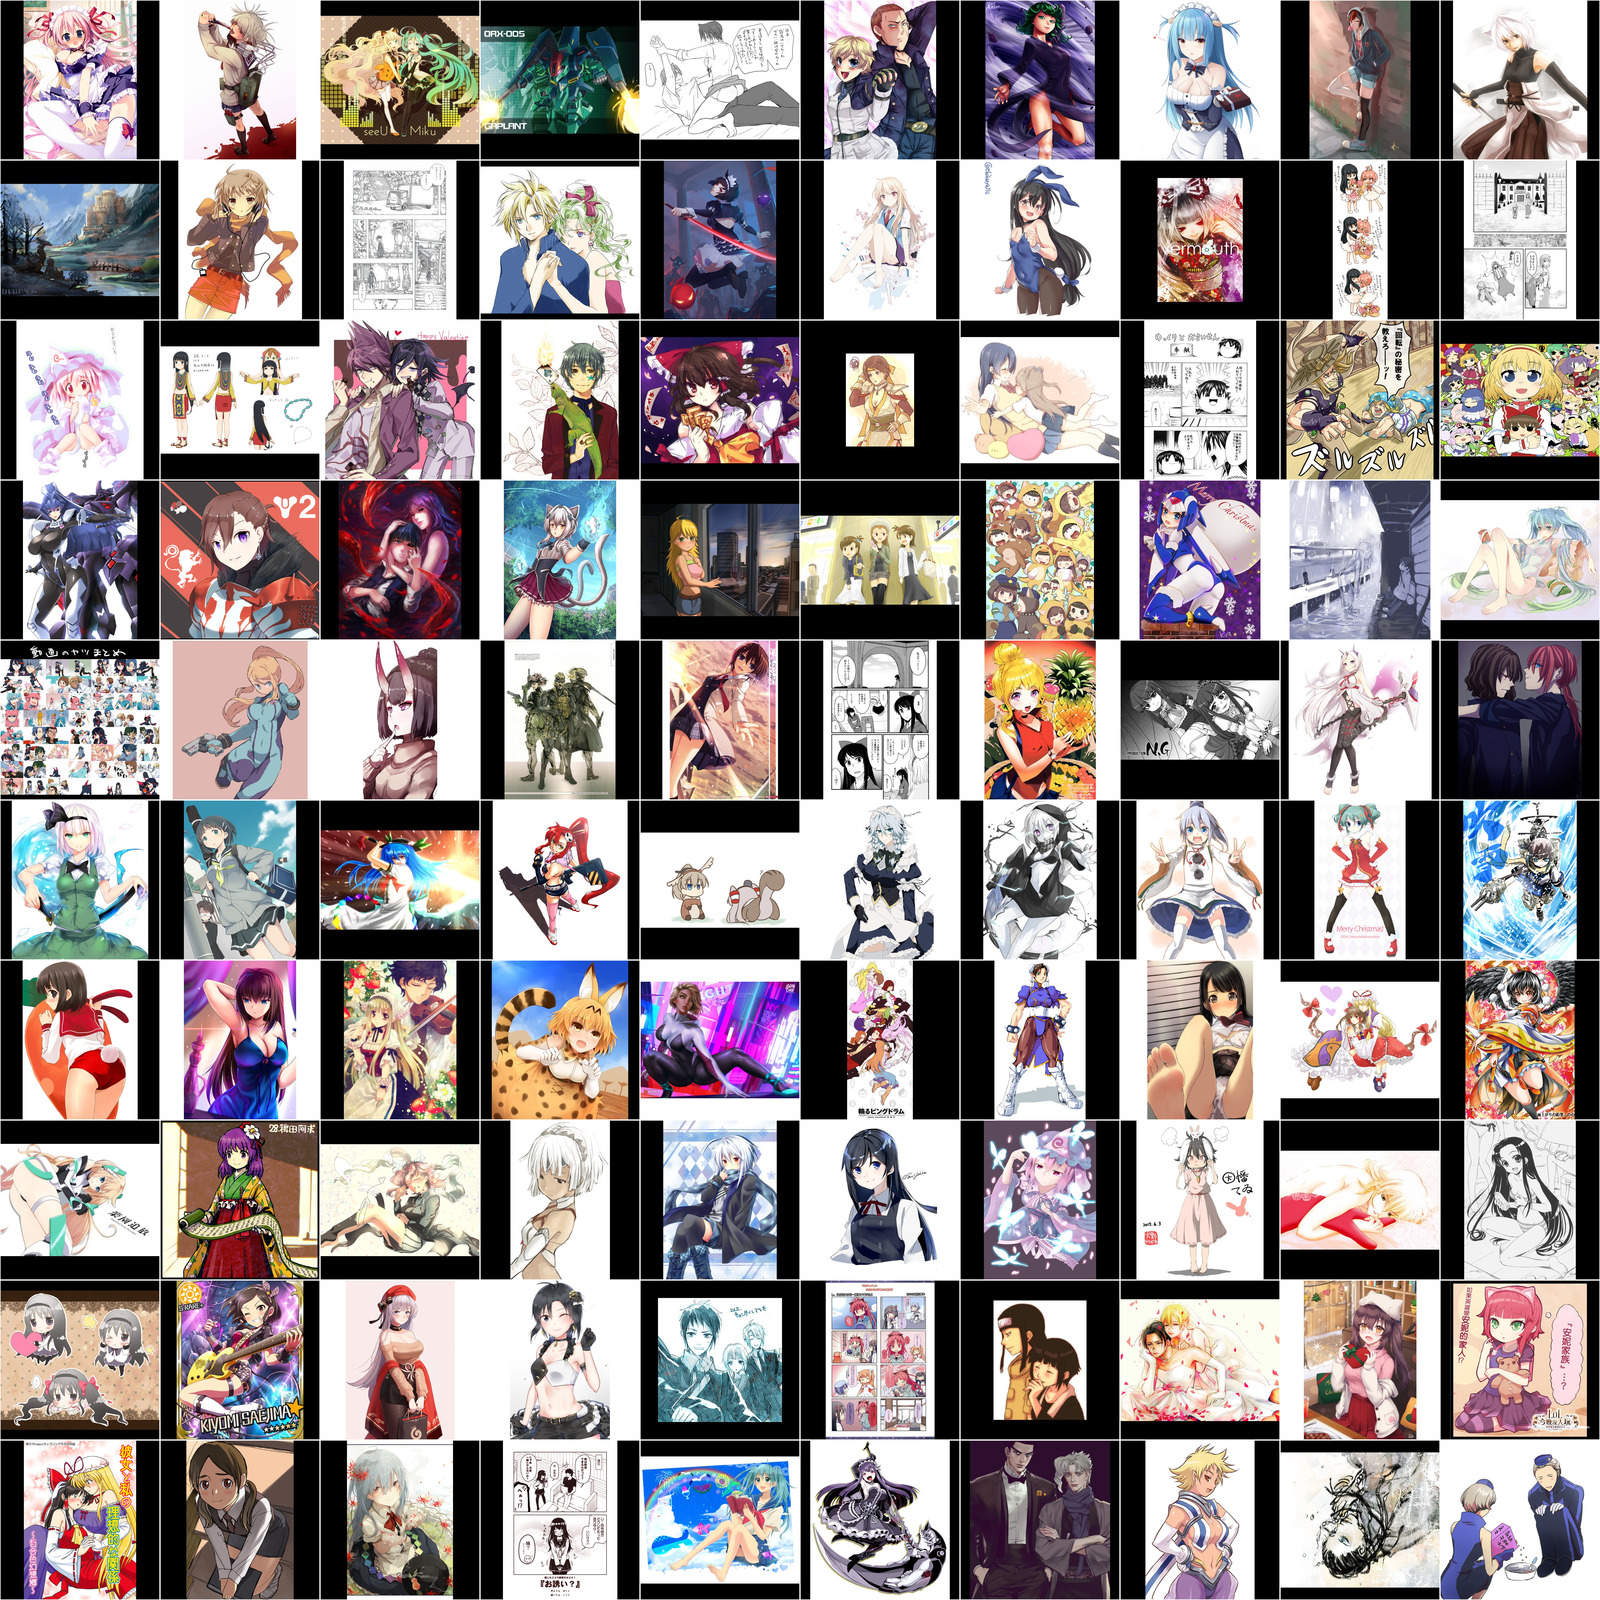
\includegraphics[scale=0.1]{danbooru2020-512px-samples.jpg}
\caption{100 sample images from the danbooru2020 dataset}
\end{figure}

\section{Proposed methods}
We approach this problem by splitting it in three components: character pose extraction, character feature extraction, and image generation. To this end, there are multiple possible methods to fufill the above components.\\
First is fine-tuning a stable diffusion model using ControlNet proposed by Zhang et al. \cite{zhang2023adding}. By "locking" certain layers of the diffusion model, the generative feature of the model would be secured, while the features perceived by the model can be finely controled.\\
Another approach is the neural style transfer \cite{gatys2015neural} mentioned above. We note that the output image has similar colors as the style image, while the outline of the output image is similar to that of the input image. Since characters usually are aligned similarly (e.g. head on top, legs on bottom), we hoped that this would translate to a coherent result.\\
Last but not least, the human-focused pose transfer could be adopted for character drawings too. However, due to difference in photos of actual humans and drawings of characters, another method would need to be developed or fine-tuned for our task.

\section{Preliminary results}
Given the nature of the task, we initially attempted to fine-tune the \texttt{waifu-diffusion} diffusion model provided by hakurei on huggingface \cite{waifu-diffusion} using ControlNet. However, due to hardware limitations, this proved to be infeasible.\\
We then attempted to approach it on a painting-oriented approach of style transfer, given the drawn nature of our dataset.
\begin{figure}[h!]
\centering
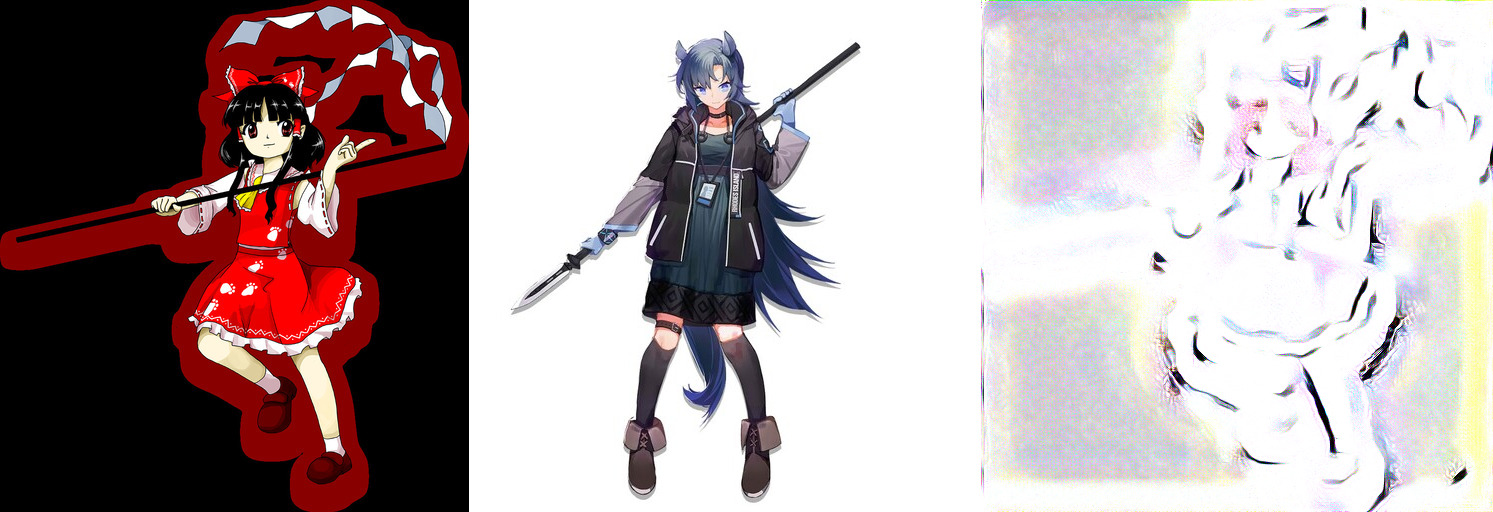
\includegraphics[scale=0.3]{final-output.jpg}
\caption{From left to right: content image, style image, output}
\label{fig2}
\end{figure}
While the outline of the output image resembles the content image, and colors are distributed roughly according to the style image (pink-ish color on the top, blue at the "torso" and "leg" parts), it does not resemble any of the two characters.\\
We plan to explore the human-based style transfer models in the next phase of the project. Should transformer-based models be unavailable due to hardware limitations, we will attempt the task with earlier GAN-based approaches.
% \end{multicols}

\bibliographystyle{IEEEtran}
\bibliography{m-report}

\end{document}
